\documentclass[tikz,border=6pt]{standalone}

\usepackage[T1]{fontenc}
\usepackage{lmodern}
\usepackage{xcolor}
\usepackage{tikz}
\usetikzlibrary{positioning,calc,arrows.meta,shadows.blur}

\definecolor{navy}{RGB}{27,54,93}
\definecolor{blue}{RGB}{73,125,209}
\definecolor{lightblue}{RGB}{232,240,255}
\definecolor{midblue}{RGB}{208,223,250}
\definecolor{green}{RGB}{40,121,92}
\definecolor{lightgreen}{RGB}{228,245,238}
\definecolor{textdark}{RGB}{33,40,52}
\definecolor{textgray}{RGB}{88,98,114}
\definecolor{lineblue}{RGB}{107,129,170}

\begin{document}
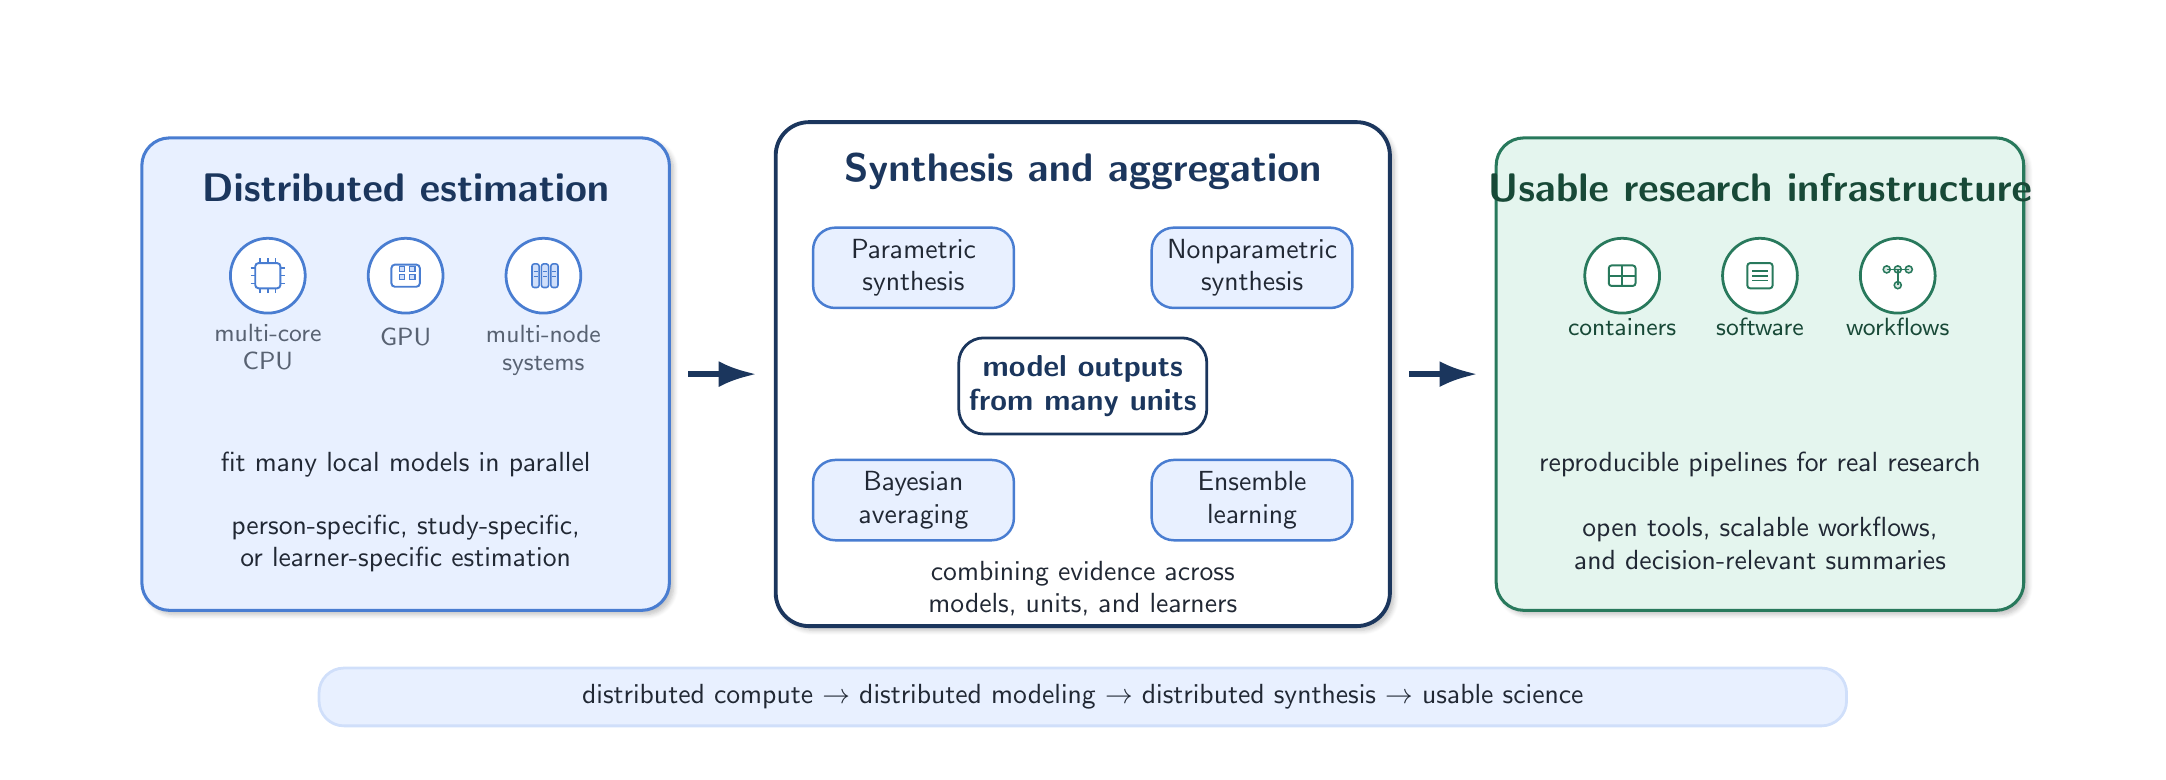
\begin{tikzpicture}[
		x=1cm,
		y=1cm,
		>=Latex,
		font=\sffamily,
		leftpanel/.style={
			rounded corners=10pt,
			draw=blue,
			line width=1.1pt,
			fill=lightblue,
			blur shadow={
				shadow blur steps=6,
				shadow xshift=1.5pt,
				shadow yshift=-1.5pt,
				shadow opacity=25
			},
			minimum width=6.7cm,
			minimum height=6.0cm,
			inner sep=0pt
		},
		centerpanel/.style={
			rounded corners=12pt,
			draw=navy,
			line width=1.4pt,
			fill=white,
			blur shadow={
				shadow blur steps=6,
				shadow xshift=1.5pt,
				shadow yshift=-1.5pt,
				shadow opacity=25
			},
			minimum width=7.8cm,
			minimum height=6.4cm,
			inner sep=0pt
		},
		rightpanel/.style={
			rounded corners=10pt,
			draw=green,
			line width=1.1pt,
			fill=lightgreen,
			blur shadow={
				shadow blur steps=6,
				shadow xshift=1.5pt,
				shadow yshift=-1.5pt,
				shadow opacity=25
			},
			minimum width=6.7cm,
			minimum height=6.0cm,
			inner sep=0pt
		},
		smallbox/.style={
			rounded corners=8pt,
			draw=blue,
			line width=0.9pt,
			fill=lightblue,
			align=center,
			inner sep=5pt,
			minimum width=2.55cm,
			minimum height=1.02cm
		},
		hubbox/.style={
			rounded corners=9pt,
			draw=navy,
			line width=1.0pt,
			fill=white,
			align=center,
			inner sep=5pt,
			minimum width=3.15cm,
			minimum height=1.22cm
		},
		strip/.style={
			rounded corners=9pt,
			draw=midblue,
			line width=1.0pt,
			fill=lightblue,
			align=center,
			inner sep=6pt
		},
		iconcircle/.style={
			circle,
			draw=blue,
			line width=1pt,
			fill=white,
			minimum size=0.95cm,
			inner sep=0pt
		},
		greeniconcircle/.style={
			circle,
			draw=green,
			line width=1pt,
			fill=white,
			minimum size=0.95cm,
			inner sep=0pt
		},
		arrow/.style={-{Latex[length=3mm,width=2.1mm]}, line width=1.1pt, draw=lineblue},
		panelarrow/.style={-{Latex[length=4.8mm,width=3.3mm]}, line width=2.1pt, draw=navy},
		smalltxt/.style={font=\sffamily\fontsize{10.0}{11.7}\selectfont, text=textdark},
		minisub/.style={font=\sffamily\fontsize{8.8}{10.2}\selectfont, text=textgray},
		paneltitle/.style={font=\sffamily\bfseries\fontsize{13.4}{15.0}\selectfont, text=navy},
		paneltitlegreen/.style={font=\sffamily\bfseries\fontsize{13.4}{15.0}\selectfont, text={green!60!black}},
		hubtitle/.style={font=\sffamily\bfseries\fontsize{10.6}{12.0}\selectfont, text=navy}
	]
	
	% Bigger canvas
	\path[draw=none] (-4.2,0.2) rectangle (22.6,9.4);
	
	% Panels spread farther apart
	\node[leftpanel]   (left)   at (0.6,5.0) {};
	\node[centerpanel] (center) at (9.2,5.0) {};
	\node[rightpanel]  (right)  at (17.8,5.0) {};
	
	% More obvious arrows between panels
	\draw[panelarrow] ($(left.east)+(0.22,0)$) -- ($(center.west)+(-0.22,0)$);
	\draw[panelarrow] ($(center.east)+(0.22,0)$) -- ($(right.west)+(-0.22,0)$);
	
	% ---------------- Left panel: Distributed estimation ----------------
	\node[paneltitle, align=center] at ($(left.north)+(0,-0.65)$)
	{Distributed estimation};
	
	\node[iconcircle] at ($(left.center)+(-1.75,1.25)$) (cpuicon) {};
	\node[iconcircle] at ($(left.center)+(0,1.25)$) (gpuicon) {};
	\node[iconcircle] at ($(left.center)+(1.75,1.25)$) (nodeicon) {};
	
	% CPU icon
	\draw[blue, line width=0.7pt, rounded corners=1.2pt]
	($(cpuicon.center)+(-0.16,-0.16)$) rectangle ($(cpuicon.center)+(0.16,0.16)$);
	\foreach \y in {-0.10,0,0.10}{
		\draw[blue, line width=0.55pt]
		($(cpuicon.center)+(-0.22,\y)$) -- ($(cpuicon.center)+(-0.16,\y)$);
		\draw[blue, line width=0.55pt]
		($(cpuicon.center)+(0.16,\y)$) -- ($(cpuicon.center)+(0.22,\y)$);
	}
	\foreach \x in {-0.10,0,0.10}{
		\draw[blue, line width=0.55pt]
		($(cpuicon.center)+(\x,0.16)$) -- ($(cpuicon.center)+(\x,0.22)$);
		\draw[blue, line width=0.55pt]
		($(cpuicon.center)+(\x,-0.22)$) -- ($(cpuicon.center)+(\x,-0.16)$);
	}
	
	% GPU icon
	\draw[blue, line width=0.7pt, rounded corners=1.2pt]
	($(gpuicon.center)+(-0.18,-0.14)$) rectangle ($(gpuicon.center)+(0.18,0.14)$);
	\foreach \dx/\dy in {-0.08/0.05,0.05/0.05,-0.08/-0.05,0.05/-0.05}{
		\filldraw[fill=midblue, draw=blue, line width=0.45pt]
		($(gpuicon.center)+(\dx,\dy)$) rectangle ++(0.07,0.07);
	}
	
	% Cluster / node icon
	\foreach \dx in {-0.10,0.02,0.14}{
		\draw[draw=blue, fill=midblue, line width=0.55pt, rounded corners=0.8pt]
		($(nodeicon.center)+(\dx-0.045,-0.15)$) rectangle ($(nodeicon.center)+(\dx+0.045,0.15)$);
		\draw[blue, line width=0.45pt]
		($(nodeicon.center)+(\dx-0.025,0.05)$) -- ($(nodeicon.center)+(\dx+0.025,0.05)$);
		\draw[blue, line width=0.45pt]
		($(nodeicon.center)+(\dx-0.025,-0.01)$) -- ($(nodeicon.center)+(\dx+0.025,-0.01)$);
	}
	
	\node[minisub, align=center] at ($(cpuicon.center)+(0,-0.9)$) {multi-core\\CPU};
	\node[minisub, align=center] at ($(gpuicon.center)+(0,-0.78)$) {GPU};
	\node[minisub, align=center] at ($(nodeicon.center)+(0,-0.95)$) {multi-node\\systems};
	
	\node[smalltxt, align=center] at ($(left.center)+(0,-1.15)$)
	{fit many local models in parallel};
	
	\node[smalltxt, align=center] at ($(left.center)+(0,-2.15)$)
	{person-specific, study-specific,\\or learner-specific estimation};
	
	% ---------------- Center panel: Synthesis and aggregation ----------------
	\node[paneltitle, align=center] at ($(center.north)+(0,-0.65)$)
	{Synthesis and aggregation};
	
	\node[hubbox] (hub) at ($(center.center)+(0,-0.15)$) {};
	\node[hubtitle, align=center] at (hub.center)
	{model outputs\\from many units};
	
	\node[smallbox] (param) at ($(center.center)+(-2.15,1.35)$) {};
	\node[smallbox] (nonparam) at ($(center.center)+(2.15,1.35)$) {};
	\node[smallbox] (bayes) at ($(center.center)+(-2.15,-1.60)$) {};
	\node[smallbox] (ensemble) at ($(center.center)+(2.15,-1.60)$) {};
	
	\node[smalltxt, align=center] at (param.center)
	{Parametric\\synthesis};
	
	\node[smalltxt, align=center] at (nonparam.center)
	{Nonparametric\\synthesis};
	
	\node[smalltxt, align=center] at (bayes.center)
	{Bayesian\\averaging};
	
	\node[smalltxt, align=center] at ($(ensemble.center)$)
	{Ensemble\\learning};
	
	% \draw[arrow] (hub.north west) -- (param.south east);
	% \draw[arrow] (hub.north east) -- (nonparam.south west);
	% \draw[arrow] (hub.south west) -- (bayes.north east);
	% \draw[arrow] (hub.south east) -- (ensemble.north west);
	
	\node[smalltxt, align=center] at ($(center.south)+(0,0.50)$)
	{combining evidence across\\models, units, and learners};
	
	% ---------------- Right panel: Usable research infrastructure ----------------
	\node[paneltitlegreen, align=center] at ($(right.north)+(0,-0.65)$)
	{Usable research infrastructure};
	
	\node[greeniconcircle] at ($(right.center)+(-1.75,1.25)$) (conticon) {};
	\node[greeniconcircle] at ($(right.center)+(0,1.25)$) (softicon) {};
	\node[greeniconcircle] at ($(right.center)+(1.75,1.25)$) (workicon) {};
	
	% Container icon
	\draw[green, line width=0.7pt, rounded corners=1pt]
	($(conticon.center)+(-0.17,-0.13)$) rectangle ($(conticon.center)+(0.17,0.13)$);
	\draw[green, line width=0.6pt]
	($(conticon.center)+(-0.17,0)$) -- ($(conticon.center)+(0.17,0)$);
	\draw[green, line width=0.6pt]
	($(conticon.center)+(0,0.13)$) -- ($(conticon.center)+(0,-0.13)$);
	
	% Software / package icon
	\draw[green, line width=0.7pt, rounded corners=1pt]
	($(softicon.center)+(-0.16,-0.16)$) rectangle ($(softicon.center)+(0.16,0.16)$);
	\draw[green, line width=0.6pt]
	($(softicon.center)+(-0.10,0.06)$) -- ($(softicon.center)+(0.10,0.06)$);
	\draw[green, line width=0.6pt]
	($(softicon.center)+(-0.10,0)$) -- ($(softicon.center)+(0.10,0)$);
	\draw[green, line width=0.6pt]
	($(softicon.center)+(-0.10,-0.06)$) -- ($(softicon.center)+(0.10,-0.06)$);
	
	% Workflow icon
	\filldraw[fill={green!18}, draw=green, line width=0.55pt]
	($(workicon.center)+(-0.14,0.08)$) circle (0.045);
	\filldraw[fill={green!18}, draw=green, line width=0.55pt]
	($(workicon.center)+(0,0.08)$) circle (0.045);
	\filldraw[fill={green!18}, draw=green, line width=0.55pt]
	($(workicon.center)+(0.14,0.08)$) circle (0.045);
	\filldraw[fill={green!18}, draw=green, line width=0.55pt]
	($(workicon.center)+(0,-0.12)$) circle (0.045);
	\draw[green, line width=0.6pt]
	($(workicon.center)+(-0.14,0.08)$) -- ($(workicon.center)+(0,0.08)$);
	\draw[green, line width=0.6pt]
	($(workicon.center)+(0,0.08)$) -- ($(workicon.center)+(0.14,0.08)$);
	\draw[green, line width=0.6pt]
	($(workicon.center)+(0,0.08)$) -- ($(workicon.center)+(0,-0.12)$);
	
	\node[minisub, align=center, text={green!60!black}] at ($(conticon.center)+(0,-0.65)$) {containers};
	\node[minisub, align=center, text={green!60!black}] at ($(softicon.center)+(0,-0.65)$) {software};
	\node[minisub, align=center, text={green!60!black}] at ($(workicon.center)+(0,-0.65)$) {workflows};
	
	\node[smalltxt, align=center] at ($(right.center)+(0,-1.15)$)
	{reproducible pipelines for real research};
	
	\node[smalltxt, align=center] at ($(right.center)+(0,-2.15)$)
	{open tools, scalable workflows,\\and decision-relevant summaries};
	
	% Bottom strip
	\node[strip, minimum width=19.4cm] at (9.2,0.90)
	{\sffamily\fontsize{10.4}{12.0}\selectfont\color{textdark}
		distributed compute $\rightarrow$ distributed modeling $\rightarrow$ distributed synthesis $\rightarrow$ usable science};
	
\end{tikzpicture}
\end{document}